\documentclass[12pt, letterpaper]{article}
\usepackage{graphicx}
\graphicspath{{images/}} 
\usepackage{titling}
\usepackage{amsmath}
\usepackage{listings}
\usepackage{xcolor}

\usepackage[margin=1in]{geometry}

\usepackage[utf8]{inputenc}
\usepackage{parallel}
\usepackage{siunitx}
\usepackage{booktabs}
\usepackage{fancyhdr}

\usepackage[export]{adjustbox}
\usepackage[margin=0.5in]{geometry}
\addtolength{\topmargin}{0in}

\usepackage{libertine}
\renewcommand*\familydefault{\sfdefault}  %% Only if the base font of the document is to be sans serif
\usepackage[T1]{fontenc}







\title{Spatial Mapping System Using Time-of-Flight}
\author{Hamza Siddiqui - 400407170 - siddih38 }
\date{\today}

%\begin{document}

\pagestyle{fancy}

\lhead{Hamza Siddiqui}
\chead {\today}
\rhead{SMSUTOF HS 2023 v0.1}


\onecolumn

\begin{figure}
\begin{minipage}{0.47\textwidth}
\centering

\includegraphics[width=.7\textwidth,left,height=.4\textwidth]{logo.png}

\end{minipage}
\hfill
\begin{minipage}{0.47\textwidth}
\raggedleft
\Huge \textbf{Spatial Mapping System using ToF v0.1}
\end{minipage}
\end{figure}


\begin{figure}
\begin{minipage}{0.47\textwidth}

\section*{Overview}
    \begin{itemize}
        \item Spatial distance measurement via ToF
        \item Serial interfacing via $\mathrm{I^2C}$
        \item Signal Preconditioning
        \item ADC
        \item Data Processing
        \item Control and Communication
    \end{itemize}


\end{minipage}
\hfill
\begin{minipage}{0.47\textwidth}
\centering
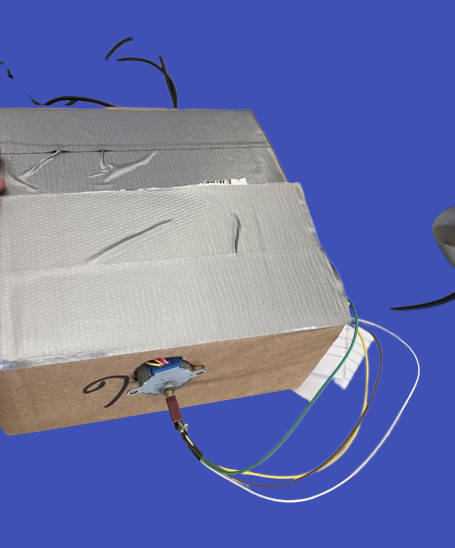
\includegraphics[width=0.7\textwidth,right]{product.jpg} %PRODUCT IMAGE PLACEHOLDER

\end{minipage}
\end{figure}





\begin{document}
\maketitle
\thispagestyle{fancy}

\newpage
\section{Device Overview}
\subsection{Features}
\subsection{General Description}
\subsection{Block Diagram (Data Flow Graph)}
\section{Device Characteristics Table}
\section{Detailed Description}
\subsection{Distance Measurement}
\subsection{Visualization}
\section{Application Example with Expected Output}
\section{User's Guide}
\section{Limitations}
\section{Circuit Schematic}
\section{Programming Logic Flowchart(s)}


\end{document}